\section{Evaluation}
\label{sec:evaluation}

The primary evaluation is an end-to-end BAS validation on isolated live Linux systems, not an
offline event-generator experiment. CALDERA executes the attack families in
Table~\ref{tab:malicious-scenarios}; \trustepisode observes only EDR/NDR telemetry and
authenticated source health. We evaluate whether the resulting episodes preserve attack
evidence and whether the five evidence-sufficiency axes in Table~\ref{tab:sufficiency} respond
faithfully under adversarial telemetry perturbations and physical collector outages. Result
cells and plots remain \tbd until the registered executions complete; no synthetic values or
confidence intervals are inserted.

\subsection{Research Questions and Evaluation Populations}
\label{sec:research-questions}

\textbf{RQ1 -- live-system validity.} Across the CALDERA scenarios in
Table~\ref{tab:malicious-scenarios}, does the label-blind builder recover the required attack
actions without excessive fragmentation, over-merge, or benign contamination?
\textbf{RQ2 -- evidence sufficiency.} Do coverage, provenance, lateness, contradiction, and
calibration states reflect the evidence actually available in each run without numerically
altering the maliciousness probability?
\textbf{RQ3 -- adversarial robustness.} Under source masking, event loss, interval removal,
delay, reordering, clock shift, duplication, and physical outage, how rapidly does performance
degrade, which faults cause explicit sufficiency transitions, and which remain silent because
authenticated health does not change?
\textbf{RQ4 -- replay and cost.} Are canonical outputs byte identical under replay, and what
throughput, latency, memory, storage, and recovery costs are observed?

The populations are disjoint views of the same registered runs. $\mathcal C_{form}$ contains
one terminal revision per surviving episode lineage at
$T_{form}=t_{run\_end}+L_{wm}+W_{rev}=t_{run\_end}+1020$ s; merged parents are removed.
$\mathcal C_{dec}^{all}$ contains the first finalized AssemblyOutcome per terminal lineage,
including supported and out-of-support AuditRecords and AssemblyFailureRecords. The scorable
inventory is
\begin{equation*}
\begin{aligned}
\mathcal C_{dec}^{score}=\{o\in\mathcal C_{dec}^{all}:&\ o\text{ is AuditRecord},\\
&o.decision\_eligible,\ P\in[0,1]\}.
\end{aligned}
\end{equation*}
After terminal insertion, the offline harness joins
$L(o)\in\{positive,negative,mixed,ambiguous\}$ by EpisodeRevision digest. Class-dependent
metrics use
\begin{equation*}
\mathcal C_{dec}^{binary}=\{o\in\mathcal C_{dec}^{score}:L(o)\in\{positive,negative\}\}.
\end{equation*}
$\mathcal C_{stream}$ retains every revision-keyed terminal outcome for sufficiency transitions,
replay equality, and cost. This separation prevents late revisions from duplicating RQ1/RQ2
candidates and prevents assembly failure from becoming hidden survivorship bias.

\subsection{CALDERA-Based Live-System Validation}
\label{sec:datasets}

The primary testbed uses CALDERA v5.3.0~\cite{caldera} as the BAS control plane, two isolated
Ubuntu 22.04 targets, and an inline Suricata gateway. Scenario commands execute against the live
process, file-system, service, and network state of the targets rather than against synthesized
logs. An instrumented endpoint wrapper records generic process start/exit observations to an
append-only spool; an independently stoppable forwarder emits label-free EDR events and
authenticated health. The inline sensor supplies NDR observations. This is a controlled
real-system validation, but it is not a production deployment or an evaluation of a commercial
EDR product.

The BAS orchestrator executes frozen no-profile Bash abilities and records action receipts in a
separate ground-truth store. CALDERA identifiers, ability metadata, receipts, and scenario labels
are excluded from the online pipeline. Every run records public software versions plus image,
configuration, parser, schema, topology, source, and hardware digests.

Table~\ref{tab:caldera-analysis-plan} specifies how the primary scenarios are analyzed. The
unchanged execution is the paired reference for each replay or outage condition. All displayed
states are placeholders until the live-system campaign completes.

\begin{table*}[t]
\caption{Planned CALDERA live-system and adversarial-robustness analysis. Each condition is
paired with the unchanged execution of the same scenario run. All result fields are pending.}
\label{tab:caldera-analysis-plan}
\centering
\scriptsize
\setlength{\tabcolsep}{3.2pt}
\begin{tabular}{p{0.15\textwidth}p{0.18\textwidth}p{0.20\textwidth}p{0.30\textwidth}p{0.08\textwidth}}
\toprule
\textbf{Analysis block} & \textbf{Paired condition} & \textbf{Primary performance readout} &
\textbf{Table~\ref{tab:sufficiency} readout} & \textbf{Status} \\
\midrule
Native BAS execution & attack-only and concurrent-benign modes & action coverage; Frag.; Merge; Contam.; episode P/R/F1 & five-axis state distribution at final revision & \tbd \\
Ranking/calibration & supported positive/negative outcomes & AUPRC; recall@10\%; Brier; NLL; eligibility rate & calibration support and provenance completeness & \tbd \\
Replay integrity stress & delay, reorder, clock shift, duplicate & paired metric change; revision count; stabilization time & lateness/provenance transitions and contradiction rate & \tbd \\
Partial telemetry & source mask, random drop, interval removal & retained action coverage; eligibility; out-of-support rate & coverage/calibration transitions and silent-loss rate & \tbd \\
Physical outage & EDR/NDR stop for 120/600 s & detection, ready, and stable-recovery times & coverage, lateness, and calibration trajectories & \tbd \\
Deterministic replay & identical input at 1/2/4/8 workers & byte equality; throughput; p50/p95/p99; peak RSS & exact equality of all five sufficiency axes & \tbd \\
\bottomrule
\end{tabular}
\end{table*}

Before a native run is sealed, the harness requires exactly one covering health interval from
both EDR instances and the NDR instance at every event-time point. Physical-outage runs omit
this gate by design so that the authenticated gap remains observable. Runs fail closed when a
manifest field is absent, a scenario action fails, or cleanup does not restore the target image.

\subsection{Ground Truth, Matching, and Labels}
\label{sec:ground-truth}

Allowlist schemas reject \path{operation_id}, \path{ability_id}, adversary/technique labels,
action receipts/windows, scenario class, and malicious labels from every online
object~\cite{kaufman2012leakage}. Each ground-truth group $g$ registers a nonempty set of required
action tokens $A_g$; each run registers benign/background tokens $B_r$. For predicted episode
$p$, $A_{cov}(p,g)=|A_p\cap A_g|/|A_g|$, where $A_p$ is its root-deduplicated attributed action
set. Offline matching constructs the threshold-qualified edge graph $E_q$. An edge requires
temporal IoU $\ge0.10$, entity Jaccard $\ge0.50$, and one exact offline receipt or registered
action. Its weight is
\begin{equation}
w=0.5A_{cov}+0.3J_{entity}+0.2\operatorname{IoU}_{time};
\quad w\ge\theta_{match}=0.50.
\label{eq:match-weight}
\end{equation}
Maximum-weight one-to-one assignment over $E_q$ operates within one run; ties use entity
overlap, absolute time difference, then ascending bytes of $(episode\_id,group\_id)$. Assignment
is used only for episode precision/recall/F1. Coverage, fragmentation, and over-merge use the
unassigned graph.

A revision chooses the first incident edge under descending $(A_{cov},w)$ then ascending group
ID. With no edge, $g^*=\texttt{null}$, $A_{cov}=0$, and $B_{cont}$ is undefined. Otherwise
\begin{equation*}
B_{cont}=\frac{|A_p\cap B_r|}{|(A_p\cap A_{g^*})\cup(A_p\cap B_r)|}.
\end{equation*}
First-match labels are mixed if $A_{cov}\ge\theta_{mal}=0.50$ and
$B_{cont}\ge\theta_{contam}=0.25$; positive if coverage passes and contamination is below the
threshold; negative if $A_{cov}=0$, a registered benign token is present, and no conflict
exists; otherwise ambiguous. Labels join only after the terminal outcome is inserted.
Sensitivity varies $\theta_{mal}\in\{.25,.50,.75\}$,
$\theta_{contam}\in\{.10,.25,.50\}$, and
$\theta_{match}\in\{.40,.50,.60\}$ without changing the primary analysis.

\begin{figure}[t]
  \centering
  \scriptsize
  \setlength{\fboxsep}{5pt}
  \begin{minipage}{\columnwidth}\centering
  \fbox{\parbox{0.91\columnwidth}{\centering
    \textbf{Online schemas reject evaluation fields}\\
    labels, receipts, windows, and scenario metadata}}\\[-1pt]
  $\downarrow$\\[-1pt]
  \fbox{\parbox{0.91\columnwidth}{\centering
    \textbf{Label-blind online pipeline}\\
    EpisodeRevision $\rightarrow$ terminal AssemblyOutcome}}\\[-1pt]
  $\downarrow$\\[-1pt]
  \fbox{\parbox{0.91\columnwidth}{\centering
    \textbf{Immutable digest join in offline harness}\\
    versioned ground truth joins only after insertion}}\\[-1pt]
  $\downarrow$\\[-1pt]
  \fbox{\parbox{0.91\columnwidth}{\centering
    \textbf{Evaluation labels and metrics}\\
    positive / negative / mixed / ambiguous}}\\[2pt]
  \textit{No evaluation field returns to inference.}
  \end{minipage}
  \caption{Ground Truth Firewall. Evaluation-only fields are rejected before inference and join
  immutable outputs only inside the offline harness.}
  \label{fig:ground-truth-firewall}
\end{figure}

\subsection{Primary BAS Scenarios}
\label{sec:scenarios}

Table~\ref{tab:malicious-scenarios} is the primary validation matrix. Each family is executed on
the live Ubuntu targets in attack-only mode and with one deterministic concurrent benign
workload. The protocol requires ten valid repetitions per family and mode; achieved counts and
all measured outcomes remain \tbd.

\begin{table*}[t]
\caption{Primary CALDERA BAS validation scenarios on live Ubuntu targets. Each card requires ten
valid repetitions in attack-only and concurrent-benign modes; achieved counts are pending.}
\label{tab:malicious-scenarios}
\centering
\scriptsize
\setlength{\tabcolsep}{3pt}
\begin{tabular}{p{0.04\textwidth}p{0.30\textwidth}p{0.17\textwidth}p{0.23\textwidth}p{0.17\textwidth}}
\toprule
\textbf{ID} & \textbf{Ordered CALDERA ability family} & \textbf{Stressor} &
\textbf{Expected EDR/NDR evidence} & \textbf{Primary sufficiency axes} \\
\midrule
M1 & discovery $\rightarrow$ peer inventory $\rightarrow$ SSH write & lateral chain & EDR lineage + NDR connection & provenance, contradiction \\
M2 & stage $\rightarrow$ archive $\rightarrow$ SCP $\rightarrow$ delayed local action & weak-to-strong & EDR file/process + NDR transfer & lateness, provenance \\
M3 & discovery $\rightarrow$ temporary-key SSH write & remote execution & EDR process + NDR session & coverage, calibration \\
M4 & five-request 60 s cadence $\rightarrow$ local action & sparse sequence & NDR cadence + EDR action & coverage, lateness \\
M5 & discovery $\rightarrow$ local configuration action & source-asymmetric case & EDR evidence; valid NDR no-detection & coverage, calibration \\
M6 & matched-tool SSH $\rightarrow$ remote write & benign-tool overlap & contextual EDR/NDR evidence & contradiction, provenance \\
M7 & actions at 0/300/3900 s & gap/span boundaries & boundary revisions and late evidence & lateness, provenance \\
\bottomrule
\end{tabular}
\end{table*}

B1--B8 cover Linux inventory, manifest-pinned package installation, file synchronization,
registered service scanning, read-only SSH administration, log collection, configuration
management, and supervisor-backed maintenance. Each benign card is run alone and as the
registered concurrent background for malicious cards. Every card fixes preconditions, exact
command templates, monotonic start offsets, fixed target paths, offline-only receipts,
postconditions, cleanup, and failure predicates. Collection or action failure remains in the
failure log but is excluded from performance estimates; cleanup failure blocks image reuse.

\subsection{Adversarial Perturbations and Physical Outage}
\label{sec:partial-telemetry}

Each valid Table~\ref{tab:malicious-scenarios} execution has an immutable unchanged replay and
deterministic adversarial children. Conditions are source masking; EDR- or NDR-specific random
drop at 5/10/25\%; removal of a 30/120/300 s interval; ingest delay of 30/120/600 s; reordering
inside 30/120/600 s buffers; event-time shifts of $-120/-30/+30/+120$ s; and duplicate root
groups at 5/10/25\%. Other-source events and the original SourceCoverage journal remain fixed,
so replay isolates data-integrity stress from health-reporting stress.

The perturbation seed is domain-separated by base run, operator, source, and dose. Before the
operator is applied, base events sort by
\begin{equation*}
(t^{event},t^{ingest},source\_instance,event\_id).
\end{equation*}
Duplicate IDs are derived from the sealed seed and original event ID; collisions invalidate the
child. These rules make every adversarial condition exactly replayable without selecting an
outcome after observing labels.

Physical outage is evaluated separately because it changes authenticated source health rather
than only event delivery. The cohort crosses source $\in\{\mathrm{EDR},\mathrm{NDR}\}$,
duration $\in\{120,600\}$ s, and ten repetitions, balanced over M1/M3/M4/M7. After two healthy
heartbeats, the selected collector is stopped and at least one scenario ability executes during
the outage. We record health detection, first parser-valid ready interval after restoration, and
the first time followed by 900 s without another revision. Detection and recovery are
right-censored when their registered observation windows expire.

For run $r$, condition $q$, and scalar metric $m$, the paired effect is
\begin{equation}
\Delta m_{r,q}=m(r,q)-m(r,0),
\label{eq:paired-robustness}
\end{equation}
where $q=0$ is the unchanged replay. For sufficiency axis $k$ with categorical states
$a,b$, the transition matrix is
\begin{equation}
T_{k,q}(a,b)=\frac{1}{N_q}\sum_{r=1}^{N_q}
\mathbf{1}[U_k(r,0)=a\land U_k(r,q)=b].
\label{eq:sufficiency-transition}
\end{equation}
For the action-coverage metric, the silent-loss rate is
\begin{equation}
SL_q=\frac{1}{N_q}\sum_{r=1}^{N_q}\mathbf{1}
[A_{cov}(r,q)<A_{cov}(r,0)\land U(r,q)=U(r,0)].
\label{eq:silent-loss}
\end{equation}
Robustness is therefore not defined as score invariance alone. Event loss with an unchanged
authenticated health journal may leave $u_{coverage}$ unchanged by construction; the analysis
reports such cases through Equation~\ref{eq:silent-loss} rather than assigning an unsupported sufficiency
transition. A desirable response can otherwise be
stable episode evidence at low dose, graceful metric degradation at higher dose, or explicit
movement to \texttt{degraded}, \texttt{unavailable}, or \texttt{out\_of\_support} when the
probability is no longer justified. Silent confidence under missing evidence is treated as a
failure.

\begin{figure*}[t]
  \centering
  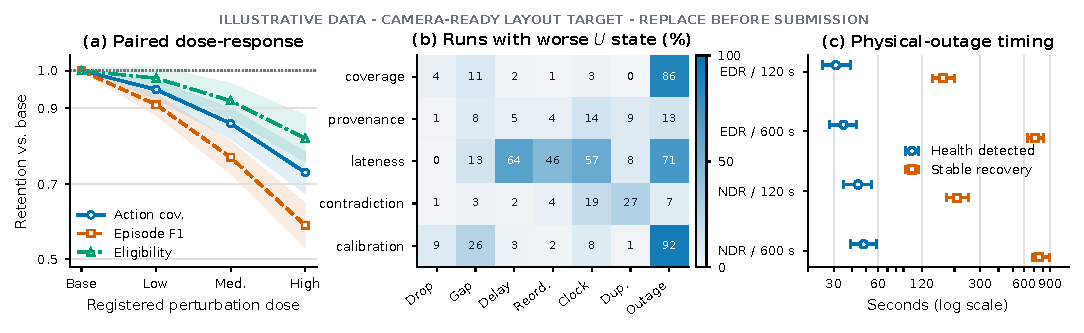
\includegraphics[width=\textwidth]{trustepisode_figures/pdf/fig10_adversarial_robustness_template.pdf}
  \caption{Illustrative camera-ready layout using simulated values, not experimental results.
  Panel (a) uses paired dose-response lines with 95\% intervals; panel (b) uses a heatmap for the
  fraction of runs moving to a worse Table~\ref{tab:sufficiency} state; panel (c) uses log-scale
  dot-and-whisker summaries for outage detection and stable recovery. All values must be replaced
  by registered measurements before submission; censored time-to-event curves belong in the
  supplementary material when censoring is material.}
  \label{fig:telemetry-perturbation-design}
\end{figure*}

\subsection{Metrics and Statistical Reporting}
\label{sec:metrics}

For run $r$, let $E_{q,r}$ be its unassigned threshold-qualified graph. For each truth group
$g$, $n_g=|\{p:(p,g)\in E_{q,r}\}|$; for episode $p$,
$d_p=|\{g:(p,g)\in E_{q,r}\}|$. Formation reporting uses run-macro action coverage,
$|G_r|^{-1}\sum_g\max(0,n_g-1)$ fragmentation,
$|P_r|^{-1}\sum_p\mathbf{1}[d_p>1]$ over-merge, mean defined contamination, and one-to-one
episode precision/recall/F1. Empty denominators are undefined, never zero.

Ranking and calibration use $\mathcal C_{dec}^{binary}$ only. AUPRC and recall among the top
$\max(1,\lceil0.10|\mathcal C_{dec,r}^{binary}|\rceil)$ per run are primary ranking metrics;
Brier, NLL, and ten-bin reliability are reported only for supported records. AUROC and
precision@$k$ are secondary~\cite{saito2015pr}. For each Table~\ref{tab:sufficiency} axis we
report state counts and proportions, the transition matrix in
Equation~\ref{eq:sufficiency-transition}, decision-eligible coverage, revision count, and time
to stable closure. Equation~\ref{eq:silent-loss} reports coverage loss not accompanied by any
sufficiency transition. Outage plots report detection, ready, and stable-recovery time with
censoring.

All summaries are macro-averaged over complete scenario runs. Paired perturbation effects use
Equation~\ref{eq:paired-robustness}; intervals use 2,000 percentile bootstrap resamples of
complete run pairs with fixed seed 20260710~\cite{field2007bootstrap}. The paper will report the
number of valid, failed, undefined, and censored runs beside every estimate. Deterministic-replay
cost is measured at 1/2/4/8 workers using one warm-up and five measured repeats, with byte
equality, throughput, ingest-to-outcome p50/p95/p99 latency, peak RSS, canonical storage bytes,
and replay time.

\subsection{External Entity-Level Context}
\label{sec:public-comparators}

Table~\ref{tab:entity-public-comparison} is secondary context, not the primary validation. It
combines entity counts reported by CAPTAIN for KAIROS, NODLINK, and CAPTAIN on DARPA TC E3
CADETS/THEIA~\cite{captain2025,kairos2024,nodlink2024} with a deterministic \trustepisode
projection. The external rows were not reproduced in this work, and the \trustepisode rows are
an entity projection from episode membership rather than a native entity classifier. HOLMES is
omitted because its reported grain is graph/campaign-level rather than an aligned E3
entity-count row~\cite{holmes2019,nodlink2024}. No cross-grain superiority claim follows.

\begin{table*}[t]
\caption{Entity-level DARPA TC E3 context. KAIROS, NODLINK, and CAPTAIN counts are transcribed
from CAPTAIN Table V~\cite{captain2025} and were not reproduced in this work. \trustepisode is
measured in this work using a deterministic projection from immutable episode membership.
Precision, recall, and F1 are derived from the displayed counts. Bold denotes the highest
precision, recall, or F1 within each dataset; ties are retained.}
\label{tab:entity-public-comparison}
\centering
\scriptsize
\setlength{\tabcolsep}{4pt}
\begin{tabular}{llrrrrrrl}
\toprule
\textbf{Dataset} & \textbf{Method} & \textbf{TP} & \textbf{FP$_{0}$} & \textbf{FN} &
\textbf{Precision} & \textbf{Recall} & \textbf{F1} & \textbf{Source} \\
\midrule
E3-CADETS & KAIROS & 15 & 1,017 & 11 & 0.015 & 0.577 & 0.028 & CAPTAIN Tbl.~V \\
 & NODLINK & 3 & 120 & 2 & 0.024 & 0.600 & 0.047 & CAPTAIN Tbl.~V \\
 & CAPTAIN & 16 & 34 & 10 & \textbf{0.320} & \textbf{0.615} & \textbf{0.421} & CAPTAIN Tbl.~V \\
 & \trustepisode & 16 & 64 & 10 & 0.200 & \textbf{0.615} & 0.302 & this work \\
\midrule
E3-THEIA & KAIROS & 12 & 3,566 & 3 & 0.003 & 0.800 & 0.007 & CAPTAIN Tbl.~V \\
 & NODLINK & 14 & 62 & 0 & 0.184 & \textbf{1.000} & 0.311 & CAPTAIN Tbl.~V \\
 & CAPTAIN & 11 & 194 & 4 & 0.054 & 0.733 & 0.100 & CAPTAIN Tbl.~V \\
 & \trustepisode & 10 & 9 & 5 & \textbf{0.526} & 0.667 & \textbf{0.588} & this work \\
\bottomrule
\end{tabular}
\end{table*}

For the reserved projection, an entity is predicted iff its canonical identifier belongs to a
decision-eligible positive terminal episode; duplicates count once per evaluation cohort. A
process-only scope aligns NODLINK, while an all-evaluable scope admits only entities in the
frozen KAIROS/CAPTAIN-aligned mapping. Projection changes no formation, score, calibration, or
threshold.

\subsection{Pending Evidence and Limitations}
\label{sec:results}
\label{sec:discussion}

The paper-facing CALDERA table and robustness figure intentionally retain \tbd markers until all
scenario repetitions, perturbation pairs, and outage traces pass validation. Replacement values
must include run counts, undefined/censored counts, and confidence intervals; a point estimate
alone is insufficient. The controlled environment demonstrates execution against live operating
systems and real EDR/NDR collection paths, but cannot establish production generalization,
unseen-evasion robustness, or field base rates. Calibration claims apply only to exact supported
manifests. The study excludes CTI, agentic response, impact/priority, OT/ICS, and autonomous
remediation.
